\section{Results}

\begin{figure}[t]
    \centering
    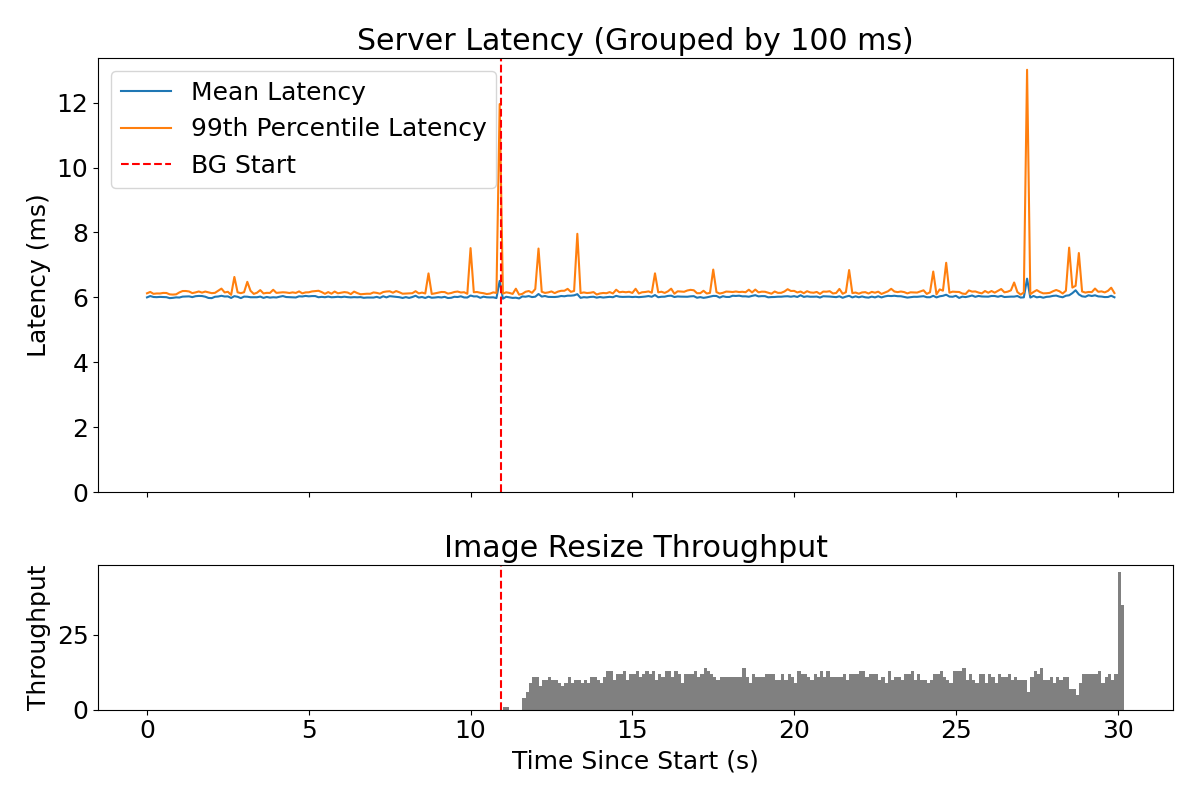
\includegraphics[width=\columnwidth]{graphs/srv-bg-schedbe-low.png}
    \caption{ \beclass{} does a good job of isolating the server's latencies
     from the load from best effort jobs}\label{fig:srv-bg-schedbe}
\end{figure}

We run the microbenchmark experiment from \autoref{fig:srv-bg-weight-cmp} using
\beclass{}. We can see the resulting performance in
\autoref{fig:srv-bg-schedbe}. As desired, the latency of the server remains
stable after the background tasks start, and the background task still runs (but
only in gaps where the core would otherwise be idle)

\begin{figure}[t]
    \centering
    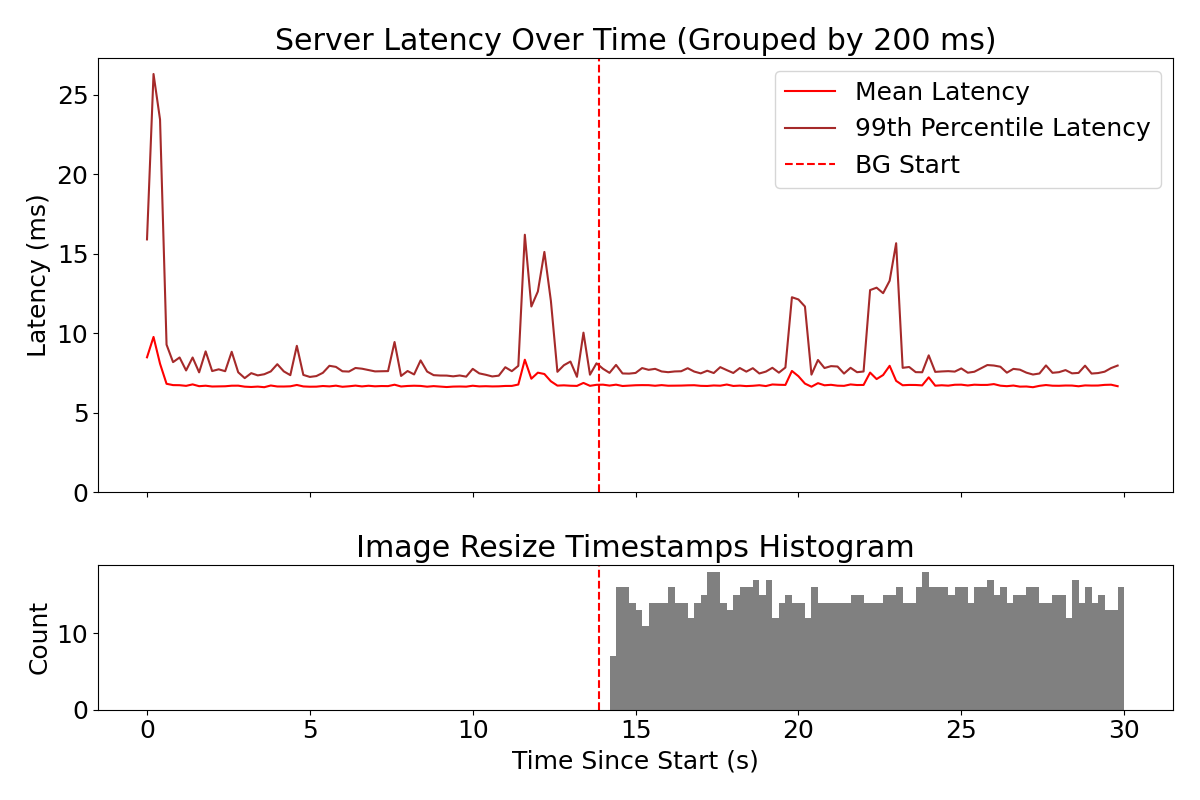
\includegraphics[width=\columnwidth]{graphs/kubernetes-schedbe.png}
    \caption{The same experiment as in \autoref{fig:kubernetes-unedited}, but
    running the BE as a \beclass{} task}\label{fig:kubernetes-schedbe}
\end{figure}

We also run the Kubernetes application from \autoref{fig:kubernetes-unedited}
using \beclass{}. The results are in \autoref{fig:kubernetes-schedbe}. We can
see that the baseline mean latency of the LC server stays around 7.4ms after
starting the the BE image resizing.

\begin{figure}[t]
    \centering
    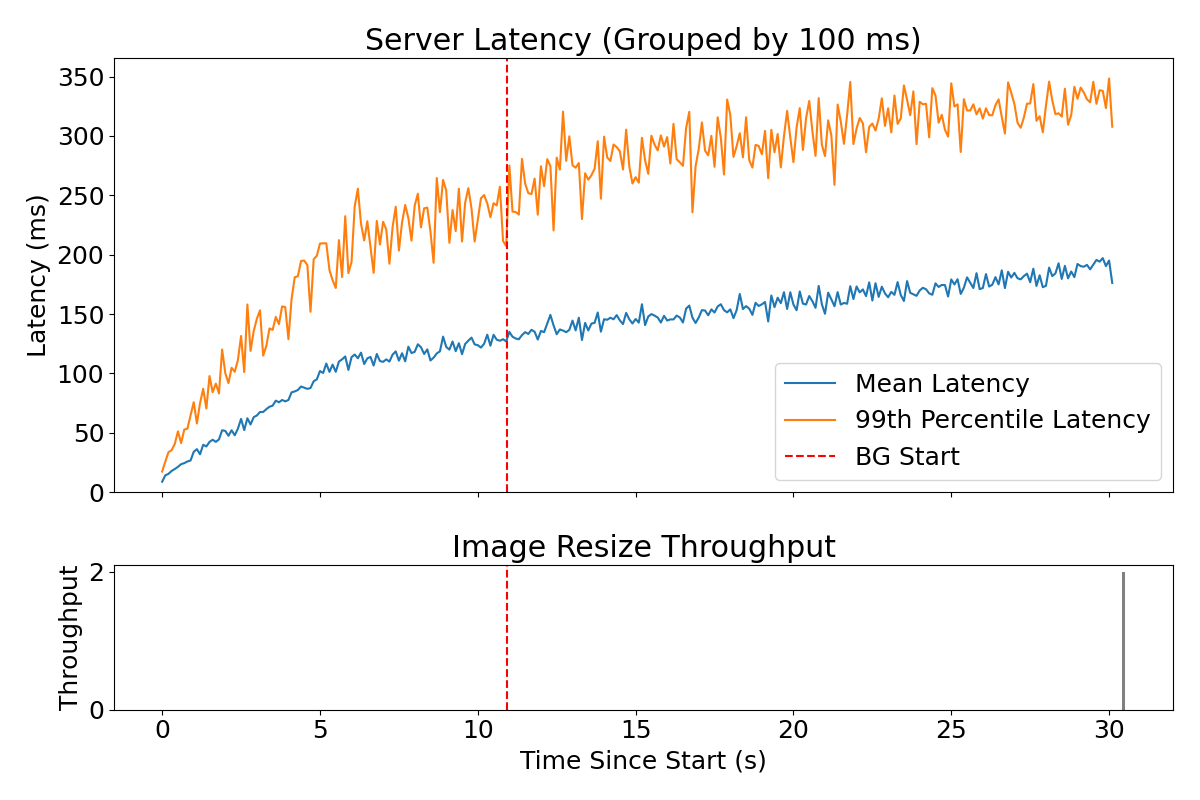
\includegraphics[width=\columnwidth]{graphs/overload-schedbe.png}
    \caption{ \beclass{} starves the BE user-space threads, leaving all CPU time
    to the LC}\label{fig:overload-schedbe}
\end{figure}

\autoref{fig:overload-schedbe} shows how parking enables the latency critical
server to keep its reservation even under sustained extremely high load. We run
the same client load as \autoref{fig:overload-rt}, but now instead instead of
throttling the server, \beclass{} parks the best effort processes. Notice that
the \beclass{} image resize job does not make progress until the very end, when
the server is done processing the requests.
